
\renewcommand{\mydate}{2025年04月24号\ 第十八次课}

%\setcounter{framenumber}{30}
\makeatletter
\ifodd\value{page}
\else
\begin{frame}[plain]
\end{frame}
\fi
\makeatother


\section{线性映射}


\title{第七章 \quad 线性映射}
\author{}
\date{}

\frame{\titlepage}

\subsection{线性映射}


\subsubsection{数组向量空间之间的线性变换与矩阵}
\begin{frame}\frametitle{数组向量空间之间的线性变换与矩阵}
给定一个数组向量空间之间的映射$\sA\colon \bF^n\rightarrow \bF^m$.
\pp
若$\sA$满足
\begin{equation}\label{equ:linearoperator}\tag{$*$}
\begin{split}
\blue{\text{(保持加法)\quad }} &\sA(\vec{a} + \vec{b}) = \sA(\vec{a}) + \sA(\vec{b});\\
\pp
\blue{\text{(保持数乘)\quad }} &\sA(\lambda\vec{a}) = \lambda\sA(\vec{a})
\end{split}
\end{equation}
\pp
则$\sA$称为从$\bF^n$到$\bF^m$的一个\blue{线性映射}.

\pp
\bigskip
我们有如下一一对应:
\begin{center}
\fbox{
从$\bF^n$到$\bF^m$的全体线性映射 \qquad $\xleftrightarrow[\sA(\vec{x})=A\vec{x}]{\quad 1:1\quad }$ \quad $\bF^{m\times n}$ }
\end{center}
\end{frame}






\begin{frame}\frametitle{例子}

\begin{example}[伸缩变换]
$\begin{pmatrix} x\\y\\\end{pmatrix}\mapsto \begin{pmatrix} k_1x\\k_2y\\\end{pmatrix} = \begin{pmatrix} k_1&\\&k_2\\\end{pmatrix}\begin{pmatrix} x\\y\\\end{pmatrix}$.
\end{example}
\pp
\begin{example}[旋转变换]
$\begin{pmatrix} x\\y\\\end{pmatrix}\mapsto \begin{pmatrix} x\cos\theta-y\sin\theta\\x\sin\theta+y\cos\theta\\\end{pmatrix} = \begin{pmatrix} \cos\theta&-\sin\theta\\\sin\theta&\cos\theta\\\end{pmatrix}\begin{pmatrix} x\\y\\\end{pmatrix}$.
\end{example}
\pp
\begin{example}
\begin{itemize}
\item[] $\bullet$ $\begin{pmatrix}1&\\&1\end{pmatrix}$ $\leftrightarrow$ \blue{恒等变换};
\pp
\qquad $\bullet$ $\begin{pmatrix}0&\\&0\end{pmatrix}$ $\leftrightarrow$ \blue{零变换};
\pp
\item[] $\bullet$  $\begin{pmatrix}\lambda&\\&\mu\end{pmatrix}$ $\leftrightarrow$ \blue{伸缩变换};
\pp
\qquad $\bullet$  $\begin{pmatrix}\cos\theta&-\sin\theta\\\sin\theta&\cos\theta\end{pmatrix}$ $\leftrightarrow$ \blue{旋转变换};
\pp
\item[] $\bullet$  $\begin{pmatrix}1&0\\0&-1\end{pmatrix}$ $\leftrightarrow$ \blue{反射变换};
\pp
\qquad $\bullet$  $\begin{pmatrix}1&\\&0\end{pmatrix}$ $\leftrightarrow$ \blue{投射变换};
\end{itemize}
\end{example}
\end{frame}



% ========== 2023年05月09号 第19次课 线性映射在基下的矩阵 ==========
%\frame{\titlepage}





\subsubsection{一般线性空间之间的线性变换}
\begin{frame}\frametitle{一般线性空间之间的线性变换}

接下来将线性映射推广到一般的线性空间上.

\begin{definition}[线性映射,线性变换和同构]
设$V$和$W$为两个$\bF$-线性空间.\gray{(注意:这里$V$和$W$不再要求是数组向量空间,而只是一般的线性空间.)}

\begin{enumerate}
\item 若映射$\sA\colon V\rightarrow W$满足
\begin{itemize}
\item  $\sA(P_1 + P_2) = \sA( P_1) + \sA(P_2)$;
\item  $\sA(\lambda P_1) = \lambda\sA( P_1)$.
\end{itemize}
则称$\sA$为从$V$到$W$的\blue{线性映射}.
\item 若$V=W$,则称线性映射$\sA$为$V$上的一个\blue{线性变换}.
\item 若线性映射$\sA$为双射,则称$\sA$为线性空间$V$到$W$的一个\blue{同构映射}. 若两个线性空间之间存在同构映射,则称它们互相\blue{同构}.
\end{enumerate}
\end{definition}
\pp
\begin{proposition}[同构基本性质]
\begin{itemize}
\item 同构映射的逆映射也是同构映射.
\pp
\item 同构为等价关系.
\pp
\item (同一域上的)有限维线性空间同构当且仅当它们维数相同.
\end{itemize}
\end{proposition}

\end{frame}






\begin{frame}\frametitle{例子}
\pp
\begin{example}
\begin{enumerate}
\item \blue{单位变换(恒等变换)}: $\varepsilon\colon V\rightarrow V$, $x\mapsto x$;
\pp
\item \blue{零映射}: $\varepsilon\colon V\rightarrow W$, $x\mapsto 0$;
\pp
\item \blue{微分变换}:
\[\sA\colon \bF_n[x] \rightarrow \bF_n[x],\quad p(x)\mapsto \frac{\mathrm{d}}{\mathrm{d}x}p(x).\]
\pp
\item \blue{积分变换}:
\[\sA\colon C[a,b]\rightarrow C[a,b],\quad f\mapsto \int_{a}^{b}K(x,t)f(t)\mathrm{d}t\]
其中 $K(x,t)$为$[a,b]\times[a,b]$上的实值连续函数.
\pp
\item \blue{线性化变换}: 记$V$为$[a,b]$上的函数集合. \[\sA:V\rightarrow V,\quad f\mapsto (1-x)f(a)+xf(b).\]
\pp
\item \blue{矩阵对应的线性映射}: $A\in \bF^{m\times n}$. \[\sA\colon \bF^n\rightarrow \bF^m,\quad x\mapsto Ax \text{(列向量)}.\]
\end{enumerate}
\end{example}
\end{frame}






\begin{frame}\frametitle{例子与反例}
\begin{example}
\begin{enumerate}\setcounter{enumi}{6}
\item \blue{投影映射}: $\sA\colon \bF^n\rightarrow \bF^r$, $(x_1,\cdots,x_n)\mapsto (x_1,\cdots,x_r)$;
\pp
\item \blue{嵌入映射}: $\sA\colon \bF^r\rightarrow \bF^n$, $(x_1,\cdots,x_r)\mapsto (x_1,\cdots,x_r,0,\cdots,0)$;
\pp
\item $\sA\colon \bF^n\rightarrow \bF^n$, $(x_1,x_2,\cdots,x_n)\mapsto (x_n,x_{n-1},\cdots,x_1)$;
\pp
\item 设$A\in \bF^{p\times m}$以及$B\in \bF^{n\times q}$为固定矩阵,
\[\sA\colon \bF^{m\times n}\rightarrow \bF^{p\times q},\quad X\mapsto AXB.\]
\pp
\item 设$V$为$\bF$上的线性空间, $\alpha_1,\cdots,\alpha_n$为 $V$中的任意 $n$个向量.
\[\sA\colon \bF^n \rightarrow V,\quad (x_1,\cdots,x_n) \mapsto x_1\alpha_1+\cdots+x_n\alpha_n.\]
\end{enumerate}
\end{example}
\pp

\begin{example}[反例]
\begin{enumerate}
\item $\sA\colon \bC^3 \rightarrow \bC^3$,  $(x,y,z)\mapsto (x^2,xy,z^2)$ 不是$\bC$-线性的.
\pp
\item $\sA\colon \bC \rightarrow \bC$, $z\mapsto \overline{z}$ 是$\bR$-线性的但不是$\bC$-线性的.
\end{enumerate}
\end{example}
\end{frame}





\subsubsection{线性变换基本性质}
\begin{frame}\frametitle{线性变换基本性质}

\begin{proposition}[线性映射的基本性质]
设$\sA$为从$\bF$-线性空间$V$到$\bF$-线性空间$W$的线性映射.
\pp
则
\begin{enumerate}
\item $\sA(0)=0$;
\pp
\item $\sA(-\alpha) = -\sA(\alpha)$, ($\forall \alpha\in V$);
\pp
\item 设$\alpha_1,\cdots,\alpha_n$为$V$的一组基. 若$\alpha = \lambda_1\alpha_1 + \cdots + \lambda_n\alpha_n$,则
\[\sA(\alpha) = \lambda_1\sA(\alpha_1) + \cdots + \lambda_n\sA(\alpha_n).\]
\pp
\yang{即,线性映射$\sA$由$\sA(\alpha_1),\cdots,\sA(\alpha_n)$这$n$个向量唯一确定.}
\pp
\item 若$\beta_1,\cdots,\beta_m$线性相关,则$\sA{\beta_1},\cdots,\sA{\beta_m}$也线性相关.
\pp
\item 若$\sA{\beta_1},\cdots,\sA{\beta_m}$线性无关,则$\beta_1,\cdots,\beta_m$也线性无关.
\end{enumerate}
\end{proposition}
\end{frame}





\subsection{线性映射与矩阵的对应}



\subsubsection{线性映射的矩阵*}
\begin{frame}\frametitle{线性映射的矩阵*}
设$\sA$为从$n$维$\bF$-向量空间$V$到$m$维$\bF$-向量空间的一个线性变换.分别取定$V$和$W$的一组基$\alpha_1,\cdots,\alpha_n$和$\beta_1,\cdots,\beta_m$.
\pp
对任意$j=1,2,\cdots,n$, 设$\sA(\alpha_j)\in W$ 在基$\beta_1,\cdots,\beta_m$下的坐标为$(a_{1j},\cdots,a_{mj})^T$,
\pp
即
\[\sA(\alpha_j) = a_{1j}\beta_1 + \cdots + a_{mj}\beta_m.\]
\pp
则这一式子可改写为
\[\blue{\sA(\alpha_1,\cdots,\alpha_n)  := \Big(\sA(\alpha_1),\cdots,\sA(\alpha_n)\Big) = (\beta_1,\cdots,\beta_m)A},\]
其中 $A:=(a_{ij})_{m\times n}\in F^{m\times n}$.
\pp
称 $A$ 为\blue{线性映射 $\sA$ 在基 $\alpha_1,\cdots,\alpha_n$和$\beta_1,\cdots,\beta_m$下的矩阵}.
\pp
\begin{example}
设$A \in\bF^{m\times n}$. 定义从$\bF^n$到$\bF^m$的线性变换
\[\sA(X) = AX.\]
则$\sA$在自然基下的矩阵为$A$.
\end{example}
\pp
\yang{证: 记$e_1,\cdots,e_n$为$\bF^n$的自然基, $e'_1,\cdots,e'_m$为$\bF^m$的自然基.则
$\sA(e_1,\cdots,e_n):=(\sA e_1,\cdots,\sA e_n)=(A e_1,\cdots,A e_n)=A(e_1,\cdots,e_n)=AI_n=A=I_mA=(e'_1,\cdots,e'_m)A$.}
\end{frame}





\begin{frame}\frametitle{线性映射的矩阵*}
\begin{example}[从矩阵出发构造线性映射]
分别取定$\bF$-线性空间$V$和$W$的一组基$\alpha_1,\cdots,\alpha_n$和$\beta_1,\cdots,\beta_m$.
\pp
对于给定矩阵$B=(b_{ij})_{m\times n}\in \bF^{m\times n}$,如下给出一个从 $V$到 $W$的映射$\sB$.
\pp
对任意的$\lambda_1\alpha_1+\cdots+\lambda_n\alpha_n\in V$, 定义\footnote{这一定义也可改写为$\sB\left((\alpha_1,\cdots,\alpha_n)\begin{pmatrix}\lambda_1\\\vdots\\\lambda_n\\\end{pmatrix}\right) = (\beta_1,\cdots,\beta_n)B\begin{pmatrix}\lambda_1\\\vdots\\\lambda_n\\\end{pmatrix}$.}
\[\sB\left(\sum_{j=1}^n\lambda_j\alpha_j\right) := \sum_{i=1}^{m} \left(\sum_{j=1}^{n} b_{ij}\lambda_j\right) \beta_i.\]
\pp
则 $\sB$为从 $V$到 $W$的一个线性映射,且其在基$\alpha_1,\cdots,\alpha_n$和$\beta_1,\cdots,\beta_m$下的矩阵正好为$B$.
\end{example}
\pp
从而,我们得到如下一一对应:
\begin{center}
\fbox{
$\left\{\text{从$V$到$W$的}\atop \text{全体线性映射}\right\}$ \quad $\xleftrightarrow[1:1 \atop \sA(\alpha_1,\cdots,\alpha_n) = (\beta_1,\cdots,\beta_n)A]{\text{基} \alpha_1,\cdots,\alpha_n \atop \text{基} \beta_1,\cdots,\beta_m }$ \quad $\bF^{m\times n}$ }
\end{center}
\end{frame}





\subsubsection{线性映射的坐标表示*}
\begin{frame}\frametitle{线性映射的坐标表示*}
\begin{theorem} 设 $A$ 为线性映射 $\sA\colon V\rightarrow W$ 在基 $\alpha_1,\cdots,\alpha_n$和$\beta_1,\cdots,\beta_m$下的矩阵. \pp
若$X$为向量$v\in V$在基$\alpha_1,\cdots,\alpha_n$下的坐标,以及$Y$为$\sA(v)$在基$\beta_1,\cdots,\beta_m$下的坐标, 则
\[Y=AX.\]
\end{theorem}
\pp
换言之,线性映射的作用可以通过对坐标左乘矩阵$A$实现.
\pp
即,下图交换
\begin{equation*}
\xymatrix@C=5cm@R=2cm{
V
\ar[r]^{\text{基 }\alpha_1,\cdots,\alpha_n}_{1:1} \ar[d]^-{\sA}_{v\mapsto \sA(v)}
\ar@{}[dr]|{\tiny \blue{\sA(\alpha_1,\cdots,\alpha_n) = (\beta_1,\cdots,\beta_n)A}}
& \bF^n
\ar[d]_-{A}^{X\mapsto AX}\\
W \ar[r]^{\text{基 }\beta_1,\cdots,\beta_n}_{1:1} & \bF^m \\
}
\end{equation*}
\pp
\yang{证明思路: $\sA(v)=\sA((\alpha_1,\cdots,\alpha_n)X) = \sA(\alpha_1,\cdots,\alpha_n)\cdot X=(\beta_1,\cdots,\beta_m)A \cdot X= (\beta_1,\cdots,\beta_m) \cdot AX$.}
\end{frame}



\renewcommand{\mydate}{2025年04月29号\ 第十九次课}


\subsubsection{线性代数的核心*}
\begin{frame}\frametitle{线性代数的核心*}

\begin{table}[]
\begin{tabular}{|cc|}
\cline{1-2}
\multicolumn{2}{|c|}{几何 $\xleftrightarrow[\text{基}]{\text{坐标系}}$ 代数} \\ \cline{1-2}
\multicolumn{1}{|c|}{线性空间} & 数组空间\\ \cline{1-2}
\multicolumn{1}{|c|}{向量}   & 坐标 \\ \cline{1-2}
\multicolumn{1}{|c|}{\qquad 线性映射\qquad \qquad } & 基下矩阵 \\ \cline{1-2}
\multicolumn{1}{|c|}{内积} & 矩阵 \\ \cline{1-2}
\multicolumn{1}{|c|}{二次型} & 矩阵 \\ \cline{1-2}
\multicolumn{1}{|c|}{张量} & 由数组成的高维阵列 \\ \cline{1-2}
\multicolumn{1}{|c|}{...} & ... \\ \cline{1-2}
\end{tabular}
\end{table}

\end{frame}




\subsection{线性变换与方阵的对应}




\subsubsection{线性变换的矩阵}
\begin{frame}\frametitle{线性变换的矩阵}
现在,我们考虑$W$等于$V$的情形.

\pp \bigskip
设$\sA$为$V$上的线性变换.固定$V$的一组基$\alpha_1,\cdots,\alpha_n$. 则存在矩阵$A:=(a_{ij})_{n\times n}$使得
\[\sA(\alpha_1,\cdots,\alpha_n) = (\alpha_1,\cdots,\alpha_n)A.\]
\pp
称矩阵$A$为\blue{线性变换$\sA$在基$(\alpha_1,\cdots,\alpha_n)$下的矩阵}.
\pp

\begin{example}
设$V=\bF^{2\times 2}$.记$A=\begin{pmatrix}1&2\\3&4\end{pmatrix}\in V$. 定义$V$上的线性变换$\sA$
\[\sA(M):=AM.\]
求$\sA$在$e_{11},e_{12},e_{21},e_{22}$下的矩阵.
\end{example}
\pp

\begin{center}
\fbox{
$\left\{\text{从$V$到$V$的}\atop \text{全体线性变换}\right\}$ \quad $\xleftrightarrow[1:1 \atop \sA(\alpha_1,\cdots,\alpha_n) = (\alpha_1,\cdots,\alpha_n)A]{\text{基} \alpha_1,\cdots,\alpha_n}$ \quad $\bF^{n\times n}$ }
\end{center}
\end{frame}





\subsubsection{线性变换的坐标表示}
\begin{frame}\frametitle{线性变换的坐标表示}
向量$x$和$\sA x$在同一组基下坐标之间的关系.
\pp
\begin{theorem}
设$\sA\colon V\rightarrow V$在基$\alpha_1,\cdots,\alpha_n$下的矩阵为$A$.
\pp
若向量$x\in V$在基$\alpha_1,\cdots,\alpha_n$下的坐标$X\in \bF^n$, 向量$\sA x$在基$\alpha_1,\cdots,\alpha_n$下的坐标为 $Y\in \bF^n$,
\pp
则
\[Y=AX.\]
\end{theorem}
\pp
\begin{equation*}
\xymatrix@C=5cm@R=2cm{
V
\ar[r]^{\text{基 }\alpha_1,\cdots,\alpha_n}_{1:1} \ar[d]_-{\sA}
\ar@{}[dr]|{\tiny \sA(\alpha_1,\cdots,\alpha_n) = (\alpha_1,\cdots,\alpha_n)A}
& \bF^n
\ar[d]^-{A}\\
V \ar[r]^{\text{基 }\alpha_1,\cdots,\alpha_n}_{1:1} & \bF^n \\
}
\end{equation*}
\end{frame}






\begin{frame}\frametitle{}

\begin{example}
记 $\alpha_1=\begin{pmatrix}2\\3\\5\end{pmatrix}$, $\alpha_2=\begin{pmatrix}0\\1\\2\end{pmatrix}$, $\alpha_3=\begin{pmatrix}1\\0\\0\end{pmatrix}$,
$\beta_1=\begin{pmatrix}1\\2\\0\end{pmatrix}$, $\beta_2=\begin{pmatrix}2\\4\\-1\end{pmatrix}$, $\beta_3=\begin{pmatrix}3\\0\\5\end{pmatrix}$.
\pp
设$\sA$为$\bF^3$上线性变换满足 $\sA(\alpha_i)=\beta_i$ ($i=1,2,3$).
\pp
求
\begin{enumerate}
\item $\sA$在$\alpha_1,\alpha_2,\alpha_3$下的矩阵;
\item $\sA$在自然基下的矩阵.
\end{enumerate}
\end{example}
\pp
\yang{解答:}
\begin{enumerate}
\item \yang{$A=(\alpha_1,\alpha_2,\alpha_3)^{-1}(\beta_1,\beta_2,\beta_3)=\begin{pmatrix}
4&9&-5\\-10&-23&15\\-7&-16&13\\\end{pmatrix}$;}
\item \yang{$B=(\beta_1,\beta_2,\beta_3)(\alpha_1,\alpha_2,\alpha_3)^{-1}=\begin{pmatrix}
3&-20&11\\0&-16&10\\5&-15&7\\\end{pmatrix}$.}
\end{enumerate}

\end{frame}









% ========== 2023年05月11号 第20次课 线性映射的矩阵与相抵关系,线性变换的矩阵与相似关系,对偶空间 ==========
%\frame{\titlepage}





\subsubsection{矩阵对应的线性变换}
\begin{frame}\frametitle{矩阵对应的线性变换}
设$\alpha_1,\cdots,\alpha_n$为$n$维$\bF$-线性空间$V$的一组基.
\begin{equation*}
\xymatrix@C=2cm@R=0cm{
\text{$V$上的线性变换}
\ar[r]^{\alpha_1,\cdots,\alpha_n}_{1:1}	& \bF^{n\times n} \\
\sA \ar@{|->}[r] & \text{ $\sA$在$\alpha_1,\cdots,\alpha_n$下的矩阵}\\
?? & B \ar@{|->}[l]\\
}
\end{equation*}
反之,给定$n$阶矩阵$B=(b_{ij})_{n\times n}$,我们可以如下定义一个映射(对于任意$\alpha=x_1\alpha_1+\cdots+x_n\alpha_n\in V$)
\[\sB(\alpha):=\sum_{i=1}^n\left(\sum_{j=1}^n b_{ij}x_j\right)\alpha_i = (\alpha_1,\cdots,\alpha_n)B\begin{pmatrix}x_1\\\vdots\\x_n\end{pmatrix}\]
\begin{proposition}
映射$\sB$为$V$上的线性变换,且其在$\alpha_1,\cdots,\alpha_n$下的矩阵为$B$.
\end{proposition}
\end{frame}





\subsubsection{线性映射的运算*}
\begin{frame}\frametitle{线性映射的运算*}
设$U$, $V$和$W$为有限维$\bF$-线性空间.
\pp
\begin{enumerate}
\item \blue{(加法)} 设$\sA$和$\sB$为从$V$到$W$的两线性映射. 对任意$v\in V$,定义
\[(\sA+\sB)(v):=\sA(v)+\sB(v);\]
\pp
\item \blue{(数乘)} 设$\sA$为从$V$到$W$的线性映射. 对于任意$v\in V$,定义
\[(\lambda\sA)(v):=\lambda\sA(v);\]
\pp
\item \blue{(合成)} 设$\sA$为从$V$到$W$的线性映射,$\sB$为从$U$到$V$的线性映射. 对于任意$u \in U$,定义
\[(\sA\circ\sB)(u):=\sA\left(\sB(u)\right).\]
\end{enumerate}
\pp
\begin{proposition}
\begin{enumerate}
\item 以上三者均为线性映射的运算.即, $\sA+\sB$, $\lambda\sA$和$\sA\circ\sB$仍为线性变换.
\pp
\item 若各自取定$U$, $V$和$W$的一组基, 设$\sA$,$\sB$在这些基下的矩阵分别为$A$,$B$, 则$\sA+\sB$, $\lambda\sA$和$\sA\circ\sB$在这些基下的矩阵分别为 $A+B$, $\lambda A$ 和 $AB$.
\pp
\item 从$V$到$W$上的全体线性映射组成的集合,记为 $\blue{\mathrm{Hom}(V,W)}$, 在线性映射的加法和数乘下构成$\bF$-线性空间.
\end{enumerate}
\end{proposition}
\end{frame}




\subsubsection{多项式在线性变换处取值}
\begin{frame}\frametitle{多项式在线性变换处取值}
设$\sA$和$\sB$为$\bF$-线性空间$V$上的线性变换.
\pp
记 $\blue{\sA^0}:=\mathrm{id}(:=\varepsilon)$.
\pp
对任意正整数$k$, 定义
\[\blue{\sA^k}:=\underbrace{\sA\circ\sA\circ\cdots\circ\sA}_{k\text{次}}.\]
\pp
对于$f(x)=a_0+a_1x+\cdots+a_nx^n\in \bF[x]$,定义
\[\blue{f(\sA)} := a_0\cdot\varepsilon + a_1\sA + \cdots a_n\sA^n.\]
\pp
\begin{example}
若$\sA$在$V$的某组基$e_1,\cdots,e_n$下的矩阵为$A$.则 $f(\sA)$在基$e_1,\cdots,e_n$下的矩阵为$f(A)$.
\end{example}
\pp
更一般地, 记 $\exp(x)=1+\frac{x}{1!}+\frac{x^2}{2!}+\frac{x^3}{3!}+\cdots$.
\pp
定义
\[\exp(\sA)=\varepsilon +\frac{\sA}{1!}+\frac{\sA^2}{2!}+\frac{\sA^3}{3!}+\cdots.\]
\pp
\begin{proposition}
若$\sA\sB=\sB\sA$,则$\exp(\sA+\sB) = \exp(\sA)\exp(\sB)$.
\end{proposition}
\end{frame}




\subsection{线性函数与对偶空间*}

\subsubsection{线性函数与对偶空间*}
\begin{frame}\frametitle{线性函数与对偶空间*}
我们考虑$W=\bF$的情形.

\pp
称从$V$到$\bF$的线性映射为$V$上的\blue{线性函数}.
\pp
记
\[\blue{V^*} = \mathrm{Hom}(V,\bF) = \{f\colon V\rightarrow \bF\mid f \text{为线性函数}\}.\]
为$V$上全体线性函数组成的集合.
\pp
由线性映射的加法和数乘,我们有线性函数的加法和数乘
\begin{equation*}
\begin{split}
& (\blue{f+g})(v) := f(v) + g(v) \\
& (\blue{\lambda f})(v) := \lambda f(v) \\
\end{split}
\end{equation*}
\pp
\begin{proposition}
在线性函数的加法和数乘下, $V^*$构成$\bF$-线性空间.\pp 称之为$V$的\blue{对偶空间}.
\end{proposition}
\end{frame}


\renewcommand{\mydate}{2025年05月13号\ 第二十次课}



\subsubsection{对偶空间基本性质*}
\begin{frame}\frametitle{对偶空间基本性质*}
\pp
\begin{proposition}[对偶空间的维数与基]
\begin{itemize}
\item 对偶空间$V^*$的维数与$V$的维数相同.
\pp
\item 若$e_1,\cdots,e_n$为$V$的一组基,则$V^*$存在唯一的一组基$f_1,\cdots,f_n$满足
\[f_j(e_i)=\delta_{ij}=\left\{{1, \quad \text{若 }i=j;\atop 0,\quad \text{若 }i\neq j}\right..\]
\pp
称$f_1,\cdots,f_n$为$e_1,\cdots,e_n$的\blue{对偶基}.
\end{itemize}
\end{proposition}
\pp
我们有如下自然的\blue{取值映射(evaluation map)}:
\[ev\colon V^*\times V\rightarrow \bF; \quad (f,v)\mapsto f(v).\]
\pp
\begin{proposition}
\[ V\cong V^{**} \quad v \mapsto ev(-,v) \]
\end{proposition}
\pp
注: 若我们不要求$V$为有限维的,则映射$V\rightarrow V^{**}$仅为单射.
\end{frame}



\subsubsection{向量的逆变性与对偶向量的协变性*}
\begin{frame}\frametitle{向量的逆变性与对偶向量的协变性*}

\begin{proposition}[向量的逆变性与对偶向量的协变性]
设$e_1,\cdots,e_n$以及 $e'_1,\cdots,e'_n$为$V$为有限维$\bF$-线性空间的两组基.
\pp
设过渡矩阵为 $A$,即
\[(e'_1,\cdots,e'_n) = (e_1,\cdots,e_n)\blue{A}.\]
\pp
记这两组基的对偶基分别为$f_1,\cdots,f_n$和$f'_1,\cdots,f'_n$.
\pp
\begin{enumerate}
\item (向量的逆变性) 设$v\in V$在两组基下坐标为$X$和$X'$. 即,
\[v = (e_1,\cdots,e_n)X = (e'_1,\cdots,e'_n)X'.\]
\pp
则
\[\blue{X' = A^{-1}X} \quad \text{或} \quad \blue{(x'_1,\cdots,x'_n) = (x_1,\cdots,x_n) (A^{-1})^T}.\]
\pp
\item (对偶向量协变性) 设对偶向量$f$在两组对偶基下坐标为$Y$和$Y'$.即,
\[f  = (f_1,\cdots,f_n)Y = (f'_1,\cdots,f'_n)Y'.\]
\pp
则
\[\blue{Y' = A^TY}  \quad \text{或} \quad \blue{(y'_1,\cdots,y'_n) = (y_1,\cdots,y_n)A}.\]
\end{enumerate}
\end{proposition}
\pp
\yang{证明思路:\[(f'_1,\cdots,f'_n) = (f_1,\cdots,f_n) (A^{-1})^T.\]}
\end{frame}





\subsection{线性映射(变换)在不同基下的矩阵与相抵(相似)关系*}

\subsubsection{线性映射在不同基下的矩阵与相抵关系*}
\begin{frame}\frametitle{线性映射在不同基下的矩阵与相抵关系*}
设$\sA$为从$n$维$\bF$-向量空间$V$到$m$维$\bF$-向量空间的一个线性映射.
\pp
设线性映射 $\sA$ 在基 $\alpha_1,\cdots,\alpha_n$和$\beta_1,\cdots,\beta_m$下矩阵为$A$. 即
\[\sA(\alpha_1,\cdots,\alpha_n) = (\beta_1,\cdots,\beta_m)A.\]
\pp
设线性映射 $\sA$ 在另外两组基 $\alpha'_1,\cdots,\alpha'_n$和$\beta'_1,\cdots,\beta'_m$下矩阵为$B$. 即
\[\sA(\alpha'_1,\cdots,\alpha'_n) = (\beta'_1,\cdots,\beta'_m)B. \pp\]
\vspace{-4mm}
\begin{theorem}
记从线性空间$V$的基$\alpha_1,\cdots,\alpha_n$到基$\alpha'_1,\cdots,\alpha'_n$的过渡矩阵为$Q$,
\pp
以及从线性空间$W$的基$\beta_1,\cdots,\beta_m$到基$\beta'_1,\cdots,\beta'_m$的过渡矩阵为$P$.
\pp
则
\[B = P^{-1}AQ.\]
\end{theorem}
\pp
\yang{$\sA(\alpha'_1,\cdots,\alpha'_n)=\sA(\alpha_1,\cdots,\alpha_n)Q = (\beta_1,\cdots,\beta_m)AQ=(\beta'_1,\cdots,\beta'_m)P^{-1}AQ$.}
\pp
\begin{corollary}
线性映射在不同基下的矩阵之间相抵.
\end{corollary}
\pp
\yang{注: 反之亦然.即,相抵的矩阵是同一个线性映射在不同基下的矩阵.}
\pp

\yang{相抵标准形的几何意义？}
\end{frame}




\subsubsection{线性变换在不同基下的矩阵与相似关系}
\begin{frame}\frametitle{线性变换在不同基下的矩阵与相似关系}
\begin{theorem}
设线性空间$V$上的线性变换$\sA$在两组基$\alpha_1,\cdots,\alpha_n$和$\beta_1,\cdots,\beta_n$下的矩阵为$A$和$B$.
\pp
设$\alpha_1,\cdots,\alpha_n$到$\beta_1,\cdots,\beta_n$的过渡矩阵为$T$.
\pp
则
\[B = T^{-1}AT.\]
\end{theorem}
\pp
\begin{example}
设线性变换$\sA\colon \bF^3\rightarrow \bF^3$满足
\[\small \sA\left(
\begin{pmatrix}2\\3\\5\end{pmatrix},
\begin{pmatrix}0\\1\\2\end{pmatrix},
\begin{pmatrix}1\\0\\0\end{pmatrix}
\right)
=
\left(
\begin{pmatrix}2\\3\\5\end{pmatrix},
\begin{pmatrix}0\\1\\2\end{pmatrix},
\begin{pmatrix}1\\0\\0\end{pmatrix}
\right)
\begin{pmatrix}4&9&-5\\-1&-23&15\\-7&-16&13\end{pmatrix}.
\]
\pp
求$\sA$在基$\small \begin{pmatrix}1\\0\\1\end{pmatrix},
\begin{pmatrix}2\\1\\2\end{pmatrix},
\begin{pmatrix}-2\\0\\-1\end{pmatrix}$下的矩阵.
\end{example}
\pp
\yang{解:\tiny
$T=\begin{pmatrix}2&0&1\\3&1&0\\5&2&0\end{pmatrix}^{-1}\begin{pmatrix}1&2&-2\\0&1&0\\1&2&-1\\\end{pmatrix}$.
$C=T^{-1}\begin{pmatrix}4&9&-5\\-1&-23&15\\-7&-16&13\end{pmatrix}T = \begin{pmatrix}-10&2&3\\10&4&10\\-2&1&0\end{pmatrix}.$}
\end{frame}





\subsubsection{矩阵的相似}
\begin{frame}\frametitle{矩阵的相似}

\begin{definition}[相似]
设$A,B\in \bF^{n\times n}$为两个$n$阶方阵.
\pp
若存在可逆阵$T\in \bF^{n\times n}$使得$B=T^{-1}AT$,则称$A$与$B$\blue{相似}.
\pp
记为 $A\sim B$.
\end{definition}
\pp
\begin{proposition}
相似为等价关系.
\end{proposition}
\pp
根据相似关系,将全体$n$阶矩阵分为若干类. \blue{相似类,代表元.}

\pp
\begin{theorem}
一个线性变换在不同基下矩阵相似.
\pp
反之任意属于该相似类的矩阵,均为该线性变换在某组基下的矩阵.
\end{theorem}
\pp
\yang{证明思路:设$\sA(\alpha_1,\cdots,\alpha_n)=(\alpha_1,\cdots,\alpha_n)A$. 若 $B=T^{-1}AT$, 记$(\beta_1,\cdots,\beta_n)=(\alpha_1,\cdots,\alpha_n)T$,则 $\sA(\beta_1,\cdots,\beta_n)=(\beta_1,\cdots,\beta_n)B$.}

\pp
\blue{相似不变量.e.g.行列式,秩.}

\pp
类比于相抵关系,对相似关系我们有如下基本问题:
\pp
\begin{enumerate}
\item 两个矩阵相似充要条件
\pp
\item 相似等价类中的最简代表元
\end{enumerate}
\end{frame}









% ========== 2023年05月16号 第21次课 习题课








% ========== 2023年05月18号 第22次课 习题课








% ========== 2023年05月23号 第23次课 特征值与特征向量 ==========
%\frame{\titlepage}



\subsection{特征值与特征向量}

\subsubsection{伸缩变换与特征向量}
\begin{frame}\frametitle{伸缩变换与特征向量}

设线性变换$\sA$在基${1 \choose 0}$,${0 \choose 1}$下的矩阵为$\begin{pmatrix}\lambda&\\&\mu\end{pmatrix}$.

\pp

\begin{tikzpicture}
\draw[->](-1.5,0)--(1.5,0)node[right]{$x$};
\draw[->](0,-1.5)--(0,1.5)node[above]{$y$};
\draw(0,0)circle(1);
\node at (1.1,1.3) {$\bullet (a,b)$};
\node at (3.5,0) {$\xRightarrow{\sA}$};
\draw[->](4.5,0)--(7.5,0)node[right]{$x$};
\draw[->](6,-1.5)--(6,1.5)node[above]{$y$};
\draw(6,0) ellipse [x radius=1.2, y radius=0.6];
\node at (7.32,0.78) {$\bullet (\lambda a,\mu b)$};
\end{tikzpicture}

\blue{问题:}
\pp
\begin{enumerate}
\item 是否任意线性变换都由某组基下的各个方向伸缩给出?(答:错误.)
\pp
\item 哪些线性变换可以由某组基下的伸缩给出? 即,哪些线性变换在合适的基下为对角阵?
\end{enumerate}
\pp
为了研究回答这些问题,我们需要引入特征值和特征向量等概念.
\end{frame}





\subsubsection{线性变换的特征值,特征向量以及特征子空间}
\begin{frame}\frametitle{线性变换的特征值,特征向量以及特征子空间}
\pp
\begin{definition}[线性变换的特征值,特征向量以及特征子空间]
设$\sA$为$n$维$\bF$-向量空间$V$上的线性变换.
\pp
若存在$\lambda\in F$以及\CJKunderdot{非零}向量$\alpha\in V$,使得
\[\sA\alpha = \lambda\alpha,\]
则称$\lambda$为$\sA$的一个\blue{特征值},
\pp
称$\alpha$为属于特征值$\lambda$的一个\blue{特征向量}.
\pp
称
\[\blue{V_\sA(\lambda)} :=\ker(\sA-\lambda \varepsilon)=\{\alpha\in V\mid \sA\alpha=\lambda\alpha\}\]
为属于$\lambda$的\blue{特征子空间}.
\end{definition}

\pp
\begin{figure}
\centering
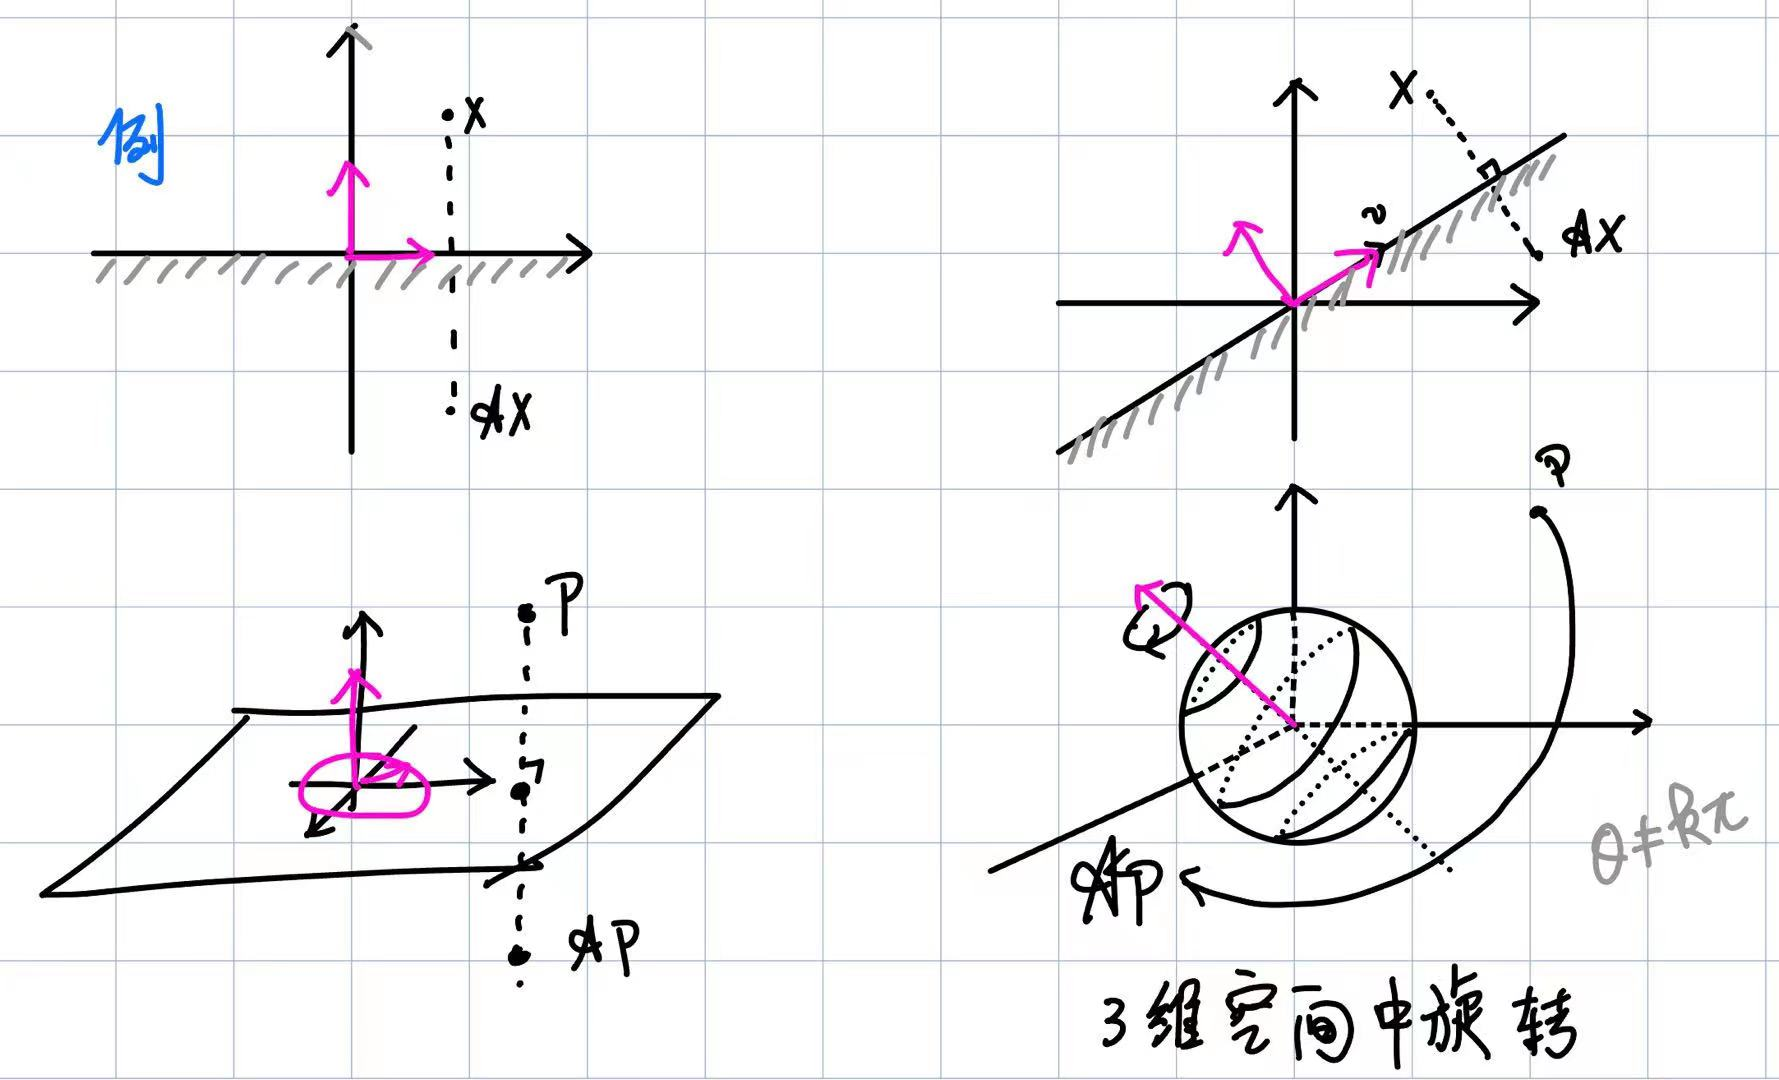
\includegraphics[width=0.6\linewidth]{pic/1e421ae12c6832e0ba34a69ad44cb6b}
\caption{}
\label{fig:1e421ae12c6832e0ba34a69ad44cb6b}
\end{figure}
\end{frame}






\subsubsection{矩阵的特征值和特征向量}
\begin{frame}\frametitle{如何求特征值和特征向量}
\blue{思路:} 通过代数(矩阵)来解决几何问题(特征值,特征向量).

\pp
设$\alpha_1,\cdots,\alpha_n$为$\bF$-线性空间$V$的一组基.
\pp
\begin{center}
\fbox{
$\left\{\text{$V$上的全体}\atop \text{线性变换}\right\}$ \quad $\xleftrightarrow[1:1 \atop \sA(\alpha_1,\cdots,\alpha_n) = (\alpha_1,\cdots,\alpha_n)A]{\text{基} \alpha_1,\cdots,\alpha_n}$ \quad $\bF^{n\times n}$ }
\end{center}
\pp
\begin{definition}[矩阵的特征值,特征向量以及特征子空间]
设$A$为$\bF$系数的$n$阶方阵.
\pp
若存在$\lambda\in F$及\CJKunderdot{非零}数组向量$x\in \bF^n$,使得
\[Ax = \lambda x,\]
\pp
则称$\lambda$为方阵$A$的\blue{特征值},
\pp
称$x$为属于特征值$\lambda$的一个\blue{特征向量}.
\pp
称
\[V_A(\lambda):=\{x\in \bF^n\mid Ax=\lambda x\}\]
为属于$\lambda$的\blue{特征子空间}.
\end{definition}
\end{frame}


\renewcommand{\mydate}{2025年05月15号\ 第二十一次课}


\subsubsection{如何求特征值和特征向量}
\begin{frame}\frametitle{如何求特征值和特征向量}
求$\sA$的特征值和特征向量可以转换为求$A$的特征值和特征向量.
\pp
\begin{proposition}
设$\alpha_1,\cdots,\alpha_n$为$\bF$-线性空间$V$的一组基.
\pp
设$V$上的线性变换在基$\alpha_1,\cdots,\alpha_n$下矩阵为$A$.
\pp
则
\begin{enumerate}
\item $\sA$与$A$有相同的特征值;
\pp
\item 若$\lambda$为$\sA$的特征值,则 $V_\sA(\lambda)=\{(\alpha_1,\cdots,\alpha_n)x\mid x\in V_A(\lambda)\}$.
\end{enumerate}
\end{proposition}
\pp
\yang{\tiny 证明思路: $x\in V_A(\lambda) \Leftrightarrow Ax=\lambda x \Leftrightarrow \sA((\alpha_1,\cdots,\alpha_n)x)=\lambda (\alpha_1,\cdots,\alpha_n)x \Leftrightarrow (\alpha_1,\cdots,\alpha_n)x\in V_{\sA}(\lambda)$.}
\pp
\begin{proposition}
设$\lambda$为方阵$A$的特征值.
\pp
则
\begin{enumerate}
\item $f(\lambda)$为$f(A)$的特征值;
\pp
特别地, $\lambda^k$为方阵$A^k$的特征值;
\pp
\item $\lambda$为方阵$A^T$的特征值;
\pp
\item 若$\lambda\neq0$,则$\frac1\lambda\det(A)$为$A^*$的特征值.
\pp
特别地,若$A$可逆,则$\frac1\lambda$为$A^{-1}$的特征值.
\pp
\item 若$A$为实矩阵且$AA^T=1$,则$|\lambda|=1$.
\end{enumerate}
\end{proposition}
\pp
注:实矩阵的特征值不一定还是实数!
\end{frame}





\subsubsection{矩阵特征值和特征向量一般求解方法}
\begin{frame}\frametitle{矩阵特征值和特征向量一般求解方法}
\begin{example}
求矩阵$A=\begin{pmatrix}1&1\\1&3\end{pmatrix}$的特征值和特征向量.
\end{example}
\pp
\yang{\tiny 解:
$A\left({x\atop y}\right)=\lambda \left({x\atop y}\right)$
\pp
$\Rightarrow$ $\begin{pmatrix}1-\lambda&1\\1&3-\lambda\\\end{pmatrix}\left({x\atop y}\right)=0$
\pp
$\Rightarrow$ $\det \begin{pmatrix}1-\lambda&1\\1&3-\lambda\\\end{pmatrix}=0$
\pp
$\Rightarrow$  $\lambda=2\pm\sqrt{2}$.

\pp
解方程组: $A\left({x\atop y}\right)= 2\pm\sqrt{2}\left({x\atop y}\right)$ 得 $\left({x\atop y}\right)=t\left({1\atop 1\pm\sqrt{2}}\right)$.
}

\pp
对于方阵$A$的特征值的计算,我们有如下一般方法:
\pp
\begin{equation*}
\begin{split}
\text{$\lambda_0$为$A$的特征值}
& \Leftrightarrow  \exists x\neq 0\quad s.t.\ Ax=\lambda_0x\\
\pp
& \Leftrightarrow  \text{线性方程组} (\lambda_0I_n-A)X=0 \text{有非零解}\\
\pp
& \Leftrightarrow  \det(\lambda_0I_n-A)=0\\
\end{split}
\end{equation*}
\pp
即,\fbox{$\lambda_0$为$A$的特征值当且仅当$\lambda_0$为多项式$\det(\lambda I_n-A)$的根.}
\pp
称行列式$\det(\lambda I-A)$为$A$的\blue{特征多项式}.记为\blue{$P_A(\lambda)$}.

\pp
\blue{注:}\begin{enumerate}
\item 数域$\bF$上的多项式在$\bF$上不一定有根!
\pp
\item (代数基本定理) 复数域$\bC$上的非常值多项式在$\bC$上一定有根.
\end{enumerate}
\pp
\yang{在计算特征值和特征向量时,总是假设$\bF=\bC$.}
\end{frame}






\begin{frame}\frametitle{矩阵特征值和特征向量一般求解方法}
设$A$为$n$阶复矩阵.求解过程分为如下两步:
\pp
\begin{enumerate}
\item 求 $P_A(\lambda)=\det(\lambda I_n - A)$,并做分解
\[P_A(\lambda) = (\lambda-\lambda_1)^{n_1}\cdot(\lambda-\lambda_2)^{n_2}\cdot\cdots\cdot(\lambda-\lambda_s)^{n_s}\]
其中$\lambda_i\in\bC$, $n_i\geq1$, $n_1+n_2+\cdots+n_s=n$.
\pp
我们称$n_i$为特征值$\lambda_i$的\blue{重数}.
\pp
\item 给定$i=1,\cdots,s$.解齐次线性方程组 $(\lambda_iI_n-A)X=0$得解空间$V_A(\lambda_i)$或者基础解系.
\end{enumerate}
\pp
\begin{example}
求矩阵$A=\begin{pmatrix}3&-1&-2\\2&0&-2\\2&-1&-1\end{pmatrix}$的特征值和特征向量.
\end{example}
\pp
\yang{答案: $P_A(\lambda)=\lambda(\lambda-1)^2$.
\pp
\begin{itemize}
\item \yang{ $(0\cdot I - A) \vec{x}=0$ $\Rightarrow$ $\vec{x}=c_1\begin{pmatrix}
1\\1\\1\\\end{pmatrix}$;}
\pp
\item \yang{$(1\cdot I - A) \vec{x}=0$ $\Rightarrow$ $\vec{x}=c_2\begin{pmatrix}
1\\2\\0\\\end{pmatrix} + c_3\begin{pmatrix}
0\\-2\\1\\\end{pmatrix}$.}
\end{itemize}
}
\end{frame}






\begin{frame}\frametitle{矩阵特征值和特征向量一般求解方法}
\begin{example}
设$A=\begin{pmatrix}1&1\\0&2\end{pmatrix}$. 设$\sA$为$V=\bF^{2\times 2}$上的线性变换满足$\sA(M)=AM$.
\pp
求$\sA$的特征值和特征向量.
\end{example}
\pp
\yang{答案: $\sA(E_{11},E_{12},E_{21},E_{22}) = (E_{11},E_{12},E_{21},E_{22})B$, 其中$B=\begin{pmatrix}
1&0&1&0\\0&1&0&1\\0&0&2&0\\0&0&0&2\\\end{pmatrix}$.
\pp
$\Rightarrow P_{\sA}(\lambda) =  P_{B}(\lambda) =(\lambda-1)^2(\lambda-2)^2$.
\pp

\begin{itemize}
\item \yang{ $(I_4 - B) \vec{x}=0$ $\Rightarrow$ 基础解系 $\begin{pmatrix}
1\\0\\0\\0\\\end{pmatrix},\begin{pmatrix}
0\\1\\0\\0\\\end{pmatrix}$
\pp
$\Rightarrow$ 特征子空间 $\langle E_{11},E_{12}\rangle$}
\pp
\item \yang{$(2I_4 - B) \vec{x}=0$ $\Rightarrow$ 基础解系$\begin{pmatrix}
1\\0\\1\\0\\\end{pmatrix},\begin{pmatrix}
0\\1\\0\\1\\\end{pmatrix}$
\pp
$\Rightarrow$ 特征子空间 $\langle E_{11}+E_{21},E_{12}+E_{22}\rangle$.}
\end{itemize}
}
\end{frame}





\subsection{相似不变量}

\subsubsection{相似不变量}
\begin{frame}\frametitle{相似不变量}
可以用矩阵来定义线性变换的哪些不变量(即,不依赖于基的选取的量).
\pp
\begin{proposition}
相似的矩阵具有相同的特征多项式和特征值.
\end{proposition}
\pp
\yang{证明:设 $B=T^{-1}AT$.则
\[P_B(\lambda)=\det(\lambda I-T^{-1}AT)=\det(T^{-1})\det(\lambda I-A)\det(T)=P_A(\lambda).\]}
\pp
即,可以用矩阵来定义线性变换的特征多项式和特征值.
\pp
有没有其它相似不变量呢?
\begin{theorem}
设$A$为$n$阶复矩阵的$n$个特征值分别为$\lambda_1,\cdots,\lambda_n$(可能有重复的).
\pp
则
\begin{enumerate}
\item $\mathrm{tr}(A)=\sum_{i=1}^{n}\lambda_i$;
\pp

\item $\det(A)=\lambda_1\lambda_2\cdots\lambda_n$.
\end{enumerate}
\end{theorem}
\pp
\yang{证明思路:展开$P_A(\lambda)$并使用根与系数之间的关系.}
\pp
\begin{corollary}
一个$n$阶方阵可逆当且仅当其$n$个特征值均不为零.
\end{corollary}
\end{frame}









% ========== 2023年05月25号 第24次课 相似对角化 ==========
%\frame{\titlepage}





\subsubsection{相似不变量的应用}
\begin{frame}\frametitle{相似不变量的应用}
\begin{example}
设$n$阶方阵$A$的全体特征值为$\lambda_1,\lambda_2,\cdots,\lambda_n$.
\pp
\begin{itemize}
\item 求$I+A$的全体特征值和行列式;
\pp
\item 更一般地,求矩阵$f(A)$的全体特征值.
\end{itemize}
\end{example}
\pp
\yang{解题思路: $P_{I+A}(\lambda)=P_A(\lambda-1)$.
\pp
 设$\lambda-f(x)=a_0\prod\limits_{i=1}^d (\alpha_i-x)$.
\pp
则
\begin{equation*} \tiny
\begin{split}
\det\left(\lambda I- f(A)\right) & = \det\left(a_0\prod_{i=1}^d(\alpha_i I-A)\right)
\pp
= a_0^n\prod_{i=1}^d\det(\alpha_i I-A) \\
\pp
& = a_0^n \prod_{i=1}^d \prod_{j=1}^n(\alpha_i-\lambda_j)
\pp
= \prod_{j=1}^n \left(a_0\prod_{i=1}^d (\alpha_i-\lambda_j)\right)
\pp
= \prod_{j=1}^n(\lambda - f(\lambda_j))\\
\end{split}
\end{equation*}
}

\pp
\begin{example}
若$A=\begin{pmatrix}1&0&0\\0&0&1\\0&1&x\end{pmatrix}$和$B=\begin{pmatrix}y&0&0\\0&-1&1\\0&0&1\end{pmatrix}$相似.求$x,y$.
\end{example}
\pp
提示:相似不变量.
\end{frame}



\subsection{相似对角化}

\subsubsection{矩阵的相似对角化}
\begin{frame}\frametitle{矩阵的相似对角化}

现在我们回到原始问题: 哪些线性变换由伸缩给出?
\pp
\begin{definition}[可对角化]
相似于对角矩阵的方阵称为\blue{可对角化}的.
\pp
我们称一个线性变换为\blue{可对角化}的,若它在某组基下的矩阵可对角化.
\end{definition}
\pp
\blue{问题:} 如何判断一个线性变换是否可对角化.
\pp
\begin{example}[不是所有的线性变换和矩阵都可对角化]
$A=\begin{pmatrix}
2&1\\0&2\\\end{pmatrix}$.
\end{example}
\end{frame}






\renewcommand{\mydate}{2025年05月20号\ 第二十二次课}



\subsubsection{可对角化的判定准则}
\begin{frame}\frametitle{可对角化的判定准则}
若 $ A=T\mathrm{diag}(\lambda_1,\cdots,\lambda_n)T^{-1}$. 记$T=(\eta_1,\cdots,\eta_n)$.
\pp
则
\begin{enumerate}
\item $\eta_1,\cdots,\eta_n$线性无关,
\pp
\item $A\eta_i=\lambda_i\eta_i$.
\end{enumerate}
\pp
\begin{theorem}[利用特征向量来判定]
方阵$A$可对角化 $\Leftrightarrow$ $A$有$n$个线性无关的特征向量.
\end{theorem}
\pp
\yang{有没有简单一点的办法来判断呢?

\pp
有时候,可以用相似不变量来判断.(不需要求特征向量!)}
\pp
\begin{lemma}
属于不同特征值的特征向量线性无关.
\pp 即,若$\lambda_1,\cdots,\lambda_k$为方阵$A$的两两不同的特征值,$\eta_i$为属于$\lambda_i$的特征向量,则$\eta_1,\cdots,\eta_k$线性无关.
\end{lemma}
\pp
\yang{证明思路:范德姆行列式不为零!}
\pp
\begin{corollary}[利用特征值来判定]
若$n$阶方阵有$n$个两两不同的特征值,则$A$可对角化.
\end{corollary}
\pp
\yang{优点:不需要求解特征向量; 缺点:不是充要条件,有重根咋办?}
\end{frame}





\subsubsection{利用重数*}
\begin{frame}\frametitle{重数*}
一般地,我们可以用特征值的重数来判定是否可对角化.
\pp
\begin{definition}[代数重数,几何重数]
设$A$为$n$阶复矩阵的特征多项式有分解
\[P_A(\lambda) = (\lambda-\lambda_1)^{n_1}(\lambda-\lambda_2)^{n_2}\cdots(\lambda-\lambda_s)^{n_s}.\]
\pp
称$n_i$为$\lambda_i$的\blue{代数重数},
\pp
称子空间$V_A(\lambda_i)$的维数为$\lambda_i$的\blue{几何重数}.
\end{definition}
\pp
\begin{theorem}[利用特征值的重数来判定]
\begin{enumerate}
\item $1\leq$ 几何重数 $\leq$ 代数重数.
\pp
\item $A$可对角化 $\Leftrightarrow$ 每个特征值的几何重数与代数重数相等.
\end{enumerate}
\end{theorem}
\pp
\yang{证明思路:将$V_A(\lambda_i)$的一组基扩充为整个空间的一组基.}
\end{frame}






\begin{frame}\frametitle{重数*}

\begin{example}
什么时候$A=\begin{pmatrix}0&0&x\\1&1&y\\1&0&0\end{pmatrix}$可对角化?
\end{example}
\pp
\yang{
解题思路: $P_A(\lambda)=(\lambda-1)(\lambda^2-x)$.
\pp
\begin{itemize}
\item \yang{$x\neq 0,1$ $\Rightarrow$ 三个不同特征值.}
\pp
\item \yang{$x=0$  $\Rightarrow$  $0$的代数重数为$2$而几何重数为$1$.}
\pp
\item \yang{$x=1$  $\Rightarrow$  $-1$的重数为$1$. $1$的代数重数为$2$,几何重数为$2$($y=-1$)或者$1$($y\neq-1$).}
\end{itemize}
}
\end{frame}



\renewcommand{\mydate}{2025年05月22号\ 第二十三次课}


\subsubsection{利用极小多项式*}
\begin{frame}\frametitle{极小多项式*}
\begin{theorem}[哈密尔顿-凯莱定理]
$P_A(A)=0$.
\end{theorem}
\pp
特别地,任意方阵$A$都存在零化多项式.称次数最小的首一零化多项式为$A$的\blue{极小多项式}.
(注:极小多项式为相似不变量.)
\pp
\begin{proposition}
\begin{enumerate}
\item 极小多项式整除其他任意零化多项式.特别地,极小多项式为特征多项式的因子.
\pp
\item 一个数为特征值当且仅当其为极小多项式的根.
\end{enumerate}
\end{proposition}
\pp
\begin{theorem}[利用极小多项式]
方阵可对角化当且仅当其极小多项式无重根.
\end{theorem}
\pp
%\yang{证明思路: 设极小多项式为$\prod\limits_{i=1}^d(x-\lambda_i)$,记 $f_j(x)=\prod\limits_{j=1\atop j\neq i}^d(x-\lambda_j)$ 以及 $V_i:=V_A(\lambda_i)$. 我们仅需证明$\bF^n=\bigoplus_{i} V_i$.
%
%存在多项式$g_1(x),\cdots,g_d(x)$使得
%$1=\sum_{j=1}^d f_i(x)g_i(x)$.
%}
\begin{corollary}[利用零化多项式]
方阵可对角化当且仅当其存在无重根的零化多项式.
\end{corollary}
\pp
\blue{例:} 设方阵 $A$满足 $A^2=A$, $A^2=I$ 或 $A^3=A$ 等.则$A$可对角化.
\end{frame}









% ========== 2023年05月30号 第25次课 上三角化,若当标准形 ==========
%\frame{\titlepage}


\subsection{相似上三角化与若当标准形}


\subsubsection{相似上三角化}
\begin{frame}\frametitle{相似上三角化}
不是每个矩阵都可以对角化,但总是可上三角化!
\pp
\begin{theorem}
\begin{enumerate}
\item 任意$n$阶复方阵$A$都相似于一个上三角形矩阵$J$,
\pp
且
\item $J$的对角线上的元素为$A$的全体特征值.
\end{enumerate}
\end{theorem}
\pp
\yang{证明思路:将$A$的一个特征向量$\xi_1$扩充为$\bC^n$的一组基$\xi_1,\cdots,\xi_n$,并记组成的可逆矩阵$(\xi_1,\cdots,\xi_n)$为$P$.
\pp
则
\[AP=P\begin{pmatrix} \lambda & * \\ & A_{22}
\end{pmatrix}.\]
\pp
对矩阵阶数归纳,不妨设$A_{22}=Q\begin{pmatrix}\lambda_2&&*\\&\ddots&\\&&\lambda_n\\\end{pmatrix}Q^{-1}$.
\pp
则
\[A= P\begin{pmatrix} 1 &  \\ & Q\end{pmatrix} \cdot \begin{pmatrix}\lambda_1&&*\\&\ddots&\\&&\lambda_n\\\end{pmatrix} \left(P\begin{pmatrix} 1 &  \\ & Q\end{pmatrix} \right)^{-1}.\]
}

\pp
\blue{注:} $J$的取法不唯一.(例:${0\ 1\choose0\ 0}$和${0\ 2\choose0\ 0}$.)

\pp
\blue{例:} 若复二阶矩阵$A$满足$A^2=0$,则$A=0$或者$A$相似于${0\ 1\choose0\ 0}$.
\end{frame}






\subsubsection{若当矩阵*}
\begin{frame}\frametitle{若当矩阵*}
相似等价类中的最简代表元是什么?
\pp
为了回答这一问题,我们需要引进:
\begin{definition}[若当块,若当矩阵]
\pp
\begin{enumerate}
\item 给定任意正整数$m$和复数$\lambda$. 称矩阵 $J_m(\lambda)=\begin{pmatrix}
\lambda&1&&\\&\lambda&\ddots&\\
&&\ddots&1\\&&&\lambda\\\end{pmatrix}$为\blue{若当块}.
\pp
\item 称由若当块组成的对角分块矩阵 $J=\begin{pmatrix}
J_{m_1}(\lambda_1)&&&\\&J_{m_2}(\lambda_2)&&\\
&&\ddots&\\&&&J_{m_s}(\lambda_s)\\\end{pmatrix}$为\blue{若当矩阵}.
\end{enumerate}
\end{definition}
\end{frame}





\subsubsection{相似等价类中的最简代表元(若当标准形)*}
\begin{frame}\frametitle{相似等价类中的最简代表元(若当标准形)*}
\begin{theorem}
\begin{enumerate}
\item 任意复方阵都与某若当矩阵相似,
\pp
并且
\item 不计若当块排序下,这个若当矩阵取法唯一.
\pp
称之为给矩阵的\blue{若当标准形}
\end{enumerate}
\end{theorem}
\pp
\begin{example}
设$\lambda$为$5$阶复矩阵$A$的$5$重特征值.请分析$A$的若当标准形.
\end{example}
\pp
\begin{example}
求矩阵$A=\begin{pmatrix}3&-2&1\\2&-2&2\\3&-6&5\end{pmatrix}$的若当标准形.
\end{example}

\yang{\[T^{-1}AT = \begin{pmatrix}2&1&\\&2&\\&&2\\\end{pmatrix}, \qquad T = \begin{pmatrix}
1 & 1 & -1 \\ 2 & 0 & 0 \\ 3 & 0 & 1 \\ \end{pmatrix}.\]}
\end{frame}





\subsubsection{若当标准形在求解常微分方程组上的一个应用*}
\begin{frame}\frametitle{若当标准形在求解常微分方程组上的一个应用*}
利用若当标准形, 可完全解决常系数线性微分方程组的求解问题.

\pp

\begin{example}
设$x,y,z$都是$t$的函数，求解常微分方程组
\begin{equation*}
\begin{cases}
\frac{\mathrm{d}x}{\mathrm{d}t}  = 3x - 2y + \ z\\
\frac{\mathrm{d}y}{\mathrm{d}t}  = 2x - 2y + 2z\\
\frac{\mathrm{d}z}{\mathrm{d}t}  = 3x - 6y + 5z\\
\end{cases}
\end{equation*}
\end{example}
\pp
\bigskip


改写原方程组为 $\frac{\mathrm{d}\mathbf{x}}{\mathrm{d}t} = A\mathbf{x}$. 作线性代换 $\mathbf{x} = T\mathbf{x}^*$, 则
\[\frac{\mathrm{d}\mathbf{x}^*}{\mathrm{d}t} = T^{-1}AT\mathbf{x}^*. \quad \text{ 即, } \quad
\begin{cases}
\frac{\mathrm{d}x^*}{\mathrm{d}t} = 2x^* + y^* \\
\frac{\mathrm{d}y^*}{\mathrm{d}t} = 2y^* \\
\frac{\mathrm{d}z^*}{\mathrm{d}t} = 2z^*
\end{cases}
\]
解此方程组得 $z^* = c_1e^{2t},\ y^* = c_2e^{2t},\ x^* = (c_2t + c_3)e^{2t}.$
再利用 $\mathbf{x} = T\mathbf{x}^*$, 即得到通解是
\[
\begin{cases}
x(t) = (c_2t + c_2 + c_3 - c_1)e^{2t} \\
y(t) = (2c_2t + 2c_3)e^{2t}  \qquad \text{其中 $c_1, c_2, c_3$ 为任意常数.}\\
z(t) = (3c_2t + 3c_3 + c_1)e^{2t}
\end{cases}
\]







\end{frame}





